\section{Export}

\subsection{Implementare}

La nivelul domeniului, funcționalitatea de export este modelată de interfața \texttt{ExportUseCase}. Aceasta definește funcțiile de listare a tuturor exporturilor de pe dispozitiv, creare a unui nou export și marcarea unui export ca finalizat la primirea unei notificări.

\lstinputlisting[style=javaCodeStyle, caption=Interfața ExportUseCase]{./code/ExportUseCase.kt}

Trimiterea datelor către cloud se face printr-un serviciu de tipul \emph{foreground}. Pe sistemul Android, \emph{serviciile foreground} sunt servicii care interacționează cu utilizatorul prin intermediul unei notificări și au șanse foarte mici de a fi oprite de către sistem pentru a recupera resurse. Acestea sunt recomandate pentru a executa activități de lungă durată care nu blochează interfața și care sunt declanșate de o acțiune a utilizatorului. Funcția \texttt{upload} este apelată într-un astfel de serviciu cu argumentul obținut pe baza formularului prezentat mai sus. La crearea argumentului \texttt{Session} este generat un id unic ce va fi folosit pentru identificarea exportului pe durata funcționării acestuia.

Interacțiunea aplicației cu serviciile cloud Firebase pentru această funcționalitate este ilustrată în diagrama din figura \ref{exportProcess}.

\begin{figure}[ht]
  \centering
  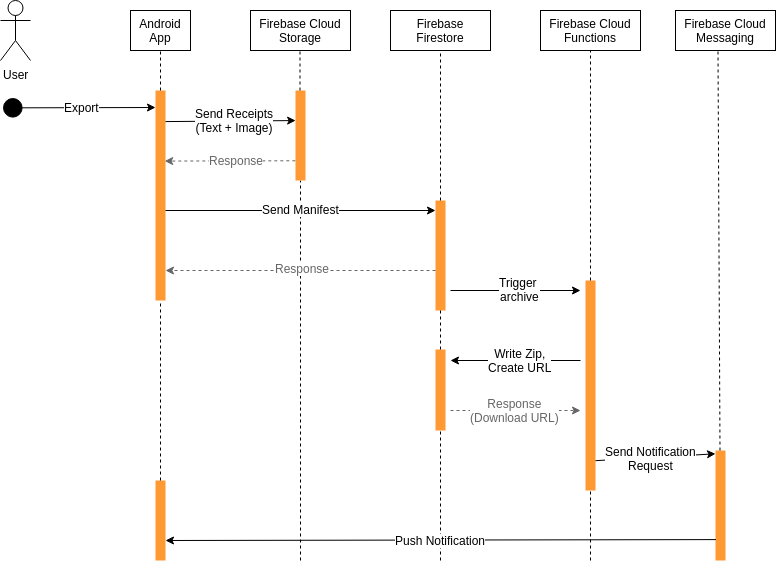
\includegraphics[width=\textwidth]{ExportSequence.png}
  \caption{Procesul de trimitere}
  \label{exportProcess}
\end{figure}

Serviciul de \emph{foreground} încarcă bonurile aferente exportului într-un spațiu de stocare \emph{Firebase Cloud Storage}, sub un folder ce are numele id-ului unic generat, în format JSON (opțional și imaginile JPEG respective). La încărcarea cu succes a acestor fișiere, obiectul \texttt{Session} este trimis ca manifest în colecția \emph{manifests} din serviciul \emph{Firebase Firestore}.

O funcție \emph{Firebase Cloud Functions} este configurată pentru a asculta schimbări ale colecției \emph{manifests} și a se declanșa la crearea unui nou obiect. Aceasta citește id-ul manifestului și opțiunea de format (JSON sau CSV) și procesează fișierele din folder-ul corespunzător din \emph{Cloud Storage}. Apoi încarcă o arhivă \emph{zip} a acestui folder în folder-ul \emph{downloads} din Cloud Sotrage și generează un link de descărcare, pe care îl trimite către serviciul \emph{Firebase Cloud Messaging} pentru a fi trimis mai departe ca notificare către dispozitiv.

Pentru ca notificarea să ajungă doar la dispozitivul care a creeat exportul, aplicația folosește clientul Android al \emph{Firebase Cloud Messaging}. Acesta presupune implementarea unui serviciu ce extinde \texttt{FirebaseMessagingService}. Acest serviciu generează un \emph{token} folosit pentru a primi notificări și îl face disponibil în metoda \texttt{onNewToken(token:\ String)}. Aplicația salvează acest token în \emph{shared preferences} și îl trimite în obiectul manifest. Astfel, acest token ajunge pe cloud, de unde este transmis către \emph{Firebase Cloud Messaging}.

\emph{Firebase Cloud Messaging} suportă două tipuri de mesaje: \emph{notification messages} și \emph{data messages}, sau o combinație dintre cele două. Pentru ca notificarea să fie gestionată imediat ce a fost primită în metoda \texttt{onMessageReceived(message:\ RemoteMessage)} a serviciului \texttt{FirebaseMessagingService}, este folosită doar funcționalitatea de \emph{data message}. Odată ce notificarea este ajunge pe dispozitiv, metoda \texttt{markAsFinished(notification:\ FinishedNotification)} este apelată pentru a actualiza baza de date și o notificare este afișată.

